\subsection{Maximising utilitarian welfare}
\label{sec:threed_sr_as_symmetric_binary_welfare}

We have shown that in an instance of 3DR-AS with binary and symmetric preferences, a stable matching must exist and can be found in polynomial time. In this section we consider a related optimisation problem, in which the goal is to find a stable matching with maximum utilitarian welfare given an instance of 3DR-AS with binary and symmetric preferences. We first show that this problem is $\NP$-hard and then extend Algorithm~\algorithmfont{findStable} to devise a $2$-approximation algorithm.

We formalise this optimisation problem as the \emph{3DR-AS Stable Maximum Utilitarian Welfare problem} (3DR-AS-SMUW). It is straightforward to show that 3DR-AS-SMUW is $\NP$-hard, as follows.

\begin{thm}
\label{thm:threed_sr_as_maxutilstable_hard}
3DR-AS-SMUW is $\NP$-hard.
\end{thm}
\begin{proof}
A direct reduction exists from PIT to the problem of deciding if a given instance of 3DR-AS-SMUW contains a stable matching $M$ with utilitarian welfare greater than or equal to a given bound, as follows. Suppose $G = (W, E)$ is an arbitrary undirected graph. First, for each vertex $w_i$ in $W$ construct one agent $\alpha_i$ in $N$. Next, for any two agents $\alpha_i, \alpha_j \in N$, let $v_{\alpha_i}(\alpha_j) = 1$ if $\{ w_i, w_j \} \in E$ and $0$ otherwise. It is straightforward to show that $(N, V)$ contains a stable matching with utilitarian welfare $2|W|$ if and only if $G$ contains a partition into triangles.
\end{proof}

Note that the reduction from PIT to 3DR-AS-SMUW also shows that the problem of finding a (not-necessarily stable) matching with maximum utilitarian welfare in a given instance of 3DR-AS is also $\NP$-hard, even when preferences are binary and symmetric.

% In Section~\ref{sec:threed_sr_as_symmetric_binary_finding_in_general} we showed that, given an arbitrary instance $(N, V)$ of 3DR-AS with binary and symmetric preferences, a stable $P$\nobreakdash-matching exists and can be found in $O(|N|^3)$ time. 

We now present an approximation algorithm for 3DR-AS-SMUW, which we call Algorithm~\algorithmfont{findStableUW}, shown in Algorithm~\ref{alg:threed_sr_as_approximationalgo}. We first provide some intuition regarding its design and then prove that it is correct and analyse its approximation ratio.

\begin{algorithm}
\textbf{Input:} an instance $(N, V)$ of 3DR-AS with binary and symmetric preferences\\
\textbf{Output:} a stable matching $M$ in $(N, V)$
\smallskip
\begin{algorithmic}
\caption{Algorithm~\algorithmfont{findStableUW}\label{alg:threed_sr_as_approximationalgo}} 
\State $M_1 \gets \algorithmfont{findStable}((N, V))$
\State $U \gets \text{agents in $N$ unmatched in $M_1$}$
\State $\mathcal{Q} \gets \algorithmfont{maximal2DMatching}((N, V), U)$
\If {$|\mathcal{Q}| \geq |U|/3 $}
    \State $\mathcal{X} \gets \text{any $|U|/3$ elements of $\mathcal{Q}$}$
\Else
    % \LineComment{Note that since $\mathcal{Q}$ is a set of disjoint pairs and $|U|\geq 1$ it follows that $|U \setminus \bigcup \mathcal{Q}|=|U|-2|\mathcal{Q}| > 2\lfloor |U|/3 \rfloor - 2|\mathcal{Q}| = 2(\lfloor |U|/3 \rfloor - |\mathcal{Q}|)$.}
    \LineComment{note that $|U \setminus \bigcup \mathcal{Q}| > 2(|U|/3 - |\mathcal{Q}|)$ since $|U \setminus \bigcup \mathcal{Q}| = |U| - 2|\mathcal{Q}|$}
\State $\mathcal{W} \gets |U|/3 - |\mathcal{Q}| \text{ pairs of agents chosen from the set of agents $U \setminus \bigcup \mathcal{Q}$}$
\State $\mathcal{X} \gets \mathcal{Q} \cup \mathcal{W}$
\EndIf
\State \textbf{end if}
\smallskip

\State $Y \gets U \setminus \bigcup \mathcal{X}$
\LineComment{Suppose $\mathcal{X}=\{X_1, X_2, \dots, X_{|U|/3}\}$ and $Y=\{y_1, y_2, \dots, y_{|U|/3}\}$. Note that $\mathcal{X}$ is a set of pairs of agents and $Y$ is a set of individual agents.}
\State $M_2 \gets \{ X_i \cup \{ y_i \} : 1 \leq i \leq |U|/3\}$
\State \Return $M_1 \cup M_2$
\end{algorithmic}
\end{algorithm}

At a high level, Algorithm~\algorithmfont{findStableUW} involves two phases. In the first phase, it calls Algorithm~\algorithmfont{findStable} to construct a stable $P$\nobreakdash-matching $M_1$. In the second phase, it orders the unmatched agents $U$ in $M_1$ into triples such that utilitarian welfare of the agents in $U$ is maximised. In order to do this, it constructs a maximal matching in the subgraph induced by $U$ and then orders the agents in $U$ to triples such that the number of triples that contain an edge in the maximal matching is maximised.

It is straightforward to show that Algorithm~\algorithmfont{findStableUW} returns a matching $M$ in polynomial time. We now analyse its approximation ratio.

Suppose $(N, V)$ is an arbitrary instance of 3DR-AS with binary and symmetric preferences, $M$ is a matching returned by Algorithm~\algorithmfont{findStableUW} given $(N, V)$ and $M^*$ is a stable matching with maximum utilitarian welfare in $(N, V)$. % Recall that $|N|=3k + l$ for some $k \geq 0$ and $0 \leq l < 3$ and by Proposition~\ref{prop:threed_sr_as_completematching} we assume that at most $l$ agents are unmatched in $M^*$ and thus that $|M^*| = k$.

At a high level, the analysis involves placing a lower bound on the welfare in $M$ of the agents in each triple apportioned by the triples in $M^*$. To do this, let $T(y)$ be the triples in $M$ with utilitarian welfare $y$ and $T^*(y)$ be the triples in $M^*$ with utilitarian welfare $y$, for some $y \geq 0$. In fact, since preferences are binary and symmetric it must be that the utilitarian welfare of any triple in $(N, V)$ must be either $0$, $2$, $4$, or $6$. Thus, by definition
\begin{align}
M &= T(6) \cup T(4) \cup T(2) \cup T(0)\label{eqn:threed_sr_as_macomposition}
\end{align}
and
\begin{align}
M^* &= T^*(6) \cup T^*(4) \cup T^*(2) \cup T^*(0)\label{eqn:threed_sr_as_moptcomposition}\enspace.
\end{align}
It follows that
% \begin{align}
%     M^* &= T^*(6) \cup T^*(4) \cup T^*(2) \cup T^*(0) \label{eqn:threed_sr_as_moptcomposition}\\
%     M &= T(6) \cup T(4) \cup T(2) \cup T(0)\label{eqn:threed_sr_as_macomposition}
% \end{align}
% \begin{alignat}{7}
%     M^* &= \matheqbox{RARoptbox}{T^*(6)} &\,& \cup &\,& \matheqbox{RARoptbox}{T^*(4)} &\,& \cup &\,& \matheqbox{RARoptbox}{T^*(2)} &\,& \cup &\,& \matheqbox{RARoptbox}{T^*(0)} \label{eqn:threed_sr_as_moptcomposition}\\
%     M &= 
%     \matheqbox{RARoptbox}{T^*(6)} &&\cup&& \matheqbox{RARoptbox}{T^*(4)} &&\cup&& \matheqbox{RARoptbox}{T^*(2)} &&\cup&& \matheqbox{RARoptbox}{T^*(0)} \label{eqn:threed_sr_as_macomposition}
% \end{alignat}
% and thus
% \begin{align}
% u(M^*) &= 6|T^*(6)| + 4|T^*(4)| + 2|T^*(2)| \label{eqn:threed_sr_as_welfareofmopt} \\
% u(M) &= 6|T^*(6)| + 4|T^*(4)| + 2|T^*(2)|\enspace. \label{eqn:threed_sr_as_bwelfareofma}
% \end{align}
\begin{align}
    u(M) &= 6|T(6)| + 4|T(4)| + 2|T(2)|\label{eqn:threed_sr_as_bwelfareofma} && \mbox{by Equation~\ref{eqn:threed_sr_as_macomposition}} 
\end{align}
and
\begin{align}
    u(M^*) &= 6|T^*(6)| + 4|T^*(4)| + 2|T^*(2)| && \mbox{by Equation~\ref{eqn:threed_sr_as_moptcomposition}.} \label{eqn:threed_sr_as_welfareofmopt}
\end{align}

We first place a lower bound on $|T(6)|$ in terms of $|T^*(6)|$.
\begin{lem}
\label{lem:threed_sr_as_tau_a_geq_tau_opt_over_3}
$|T(6)| \geq |T^*(6)|/3$.
\end{lem}
\begin{proof}
By the pseudocode of Algorithm~\algorithmfont{findStable} and the definition of Subroutine~\algorithmfont{eliminateTriangles}, $T(6)$ contains a maximal triangle packing in the underlying graph $(N, E)$. Since by definition $T^*(6)$ is also a maximal triangle packing in the same graph, it must be that $|T(6)| \geq |T^*(6)|/3$.
% Consider an arbitrary triple $\{ \alpha_{h_1}, \alpha_{h_2}, \alpha_{h_3} \} \in T^*(6)$. It must be that $v_{\alpha_{h_1}}(\alpha_{h_2})=v_{\alpha_{h_2}}(\alpha_{h_3})=v_{\alpha_{h_3}}(\alpha_{h_1})=1$. Recall that the first step of Algorithm~\algorithmfont{findStable} involved selecting a maximal set of triangles. In the pseudocode description of Algorithm~\algorithmfont{findStable}, we described this operation using Subroutine~\algorithmfont{eliminateTriangles}, which we refer to here. Since  $\{ \alpha_{h_1}, \alpha_{h_2}, \alpha_{h_3} \}$ is a triangle in $(N, V)$, either Subroutine~\algorithmfont{eliminateTriangles} selected this triple, and $\{ \alpha_{h_1}, \alpha_{h_2}, \alpha_{h_3} \} \in T^*(6)$, or at least one of $\alpha_{h_1}, \alpha_{h_2}, \alpha_{h_3}$ was added to a different triple in $T^*(6)$. In either case, any triple in $T^*(6)$ contains at least one agent that belongs to some triple in $T^*(6)$. Triples in $T^*(6)$ are disjoint, hence the number of agents in triples in $T^*(6)$ is at least $|T^*(6)|$. It follows that $|T^*(6)| \geq |T^*(6)|/3$.
\end{proof}

We now show that if no triple in $M$ has utilitarian welfare $0$ then $2u(M) \geq u(M^*)$.

\begin{lem}
\label{lem:threed_sr_as_no000exists_lem}
If $T(0) = \varnothing$ then $2{u(M)} \geq u(M^*)$.
\end{lem}
\begin{proof}
First consider $M^*$. 
% By Equation~\ref{eqn:threed_sr_as_welfareofmopt},
% \begin{align}
%     u(M^*) &= 6|T^*(6)| + 4|T^*(4)| + 2|T^*(2)|\nonumber\\
%     &\leq 6|T^*(6)| + 4(|T^*(4)| + |T^*(2)|)\nonumber\\
%     &= 6|T^*(6)| + 4(|M^*| - |T^*(6)|) && \mbox{by Equation~\ref{eqn:threed_sr_as_moptcomposition}}\nonumber\\
%     &= 6|T^*(6)| + 4(n - |T^*(6)|) && \mbox{since by definition, $|M^*|=n$}\nonumber\\
%     &= 2|T^*(6)| + 4n\label{eqn:threed_sr_as_no000exists_lem_inequality1}\enspace.
% \end{align}
Now
\begingroup
\allowdisplaybreaks
\begin{align*}
    2u(M) &= 12|T(6)| + 8|T(4)| + 4|T(2)| && \mbox{by Equation~\ref{eqn:threed_sr_as_bwelfareofma}}\\
    &\geq 12|T(6)| + 4(|T(4)| + |T(2)|)\\
    &= 12|T(6)| + 4(|M| - |T(6)|) && \mbox{by Equation~\ref{eqn:threed_sr_as_macomposition}, since $T(0)=\varnothing$}\\
    &= 12|T(6)| + 4(n - |T(6)|) && \mbox{by definition, $|M|=n$}\\
    % hack because we have code in main.tex that automatically adjusts vertical spacing
    &= 8|T(6)| + 4n\\[0.7em]
    &\geq \smash{\frac{8|T^*(6)|}{3}} + 4n && \mbox{by Lemma~\ref{lem:threed_sr_as_tau_a_geq_tau_opt_over_3}}\\[0.4em]
    &\geq 2|T^*(6)| + 4n\\
    &= 6|T^*(6)| - 4|T^*(6)| + 4n\\
    &= 6|T^*(6)| + 4(n - |T^*(6)|)\\
    &= 6|T^*(6)| + 4(|M^*| - |T^*(6)|)\\
    &= 6|T^*(6)| + 4(|T^*(4)| + |T^*(2)| + |T^*(0)|) && \mbox{by Equation~
    \ref{eqn:threed_sr_as_moptcomposition}}\\
    &= 6|T^*(6)| + 4|T^*(4)| + 4|T^*(2)| && \mbox{since $u(T^*(0))=0$}\\
    &\geq 6|T^*(6)| + 4|T^*(4)| + 2|T^*(2)|\\
    &= u(M^*) && \mbox{by Equation~\ref{eqn:threed_sr_as_welfareofmopt}.}
\end{align*}
\endgroup
\end{proof}
We now consider the case when there exists at least one triple in $T(0)$. The existence of such a triple allows us to deduce that $|\mathcal{Q}| < |U|/3$ and thus that any two agents that form an edge in the maximal matching $\mathcal{Q}$ must be assigned to the same triple in $M$.

\begin{lem}
\label{lem:threed_sr_as_approx_if000thentisnotcomplete}
If $|T(0)| > 0$ then $|\mathcal{Q}| < |U|/3$.
\end{lem}
\begin{proof}
We prove the contrapositive. Suppose $|\mathcal{Q}| \geq |U|/3$. By the pseudocode of Algorithm~\algorithmfont{findStableUW}, $\mathcal{X}\subseteq \mathcal{Q}$ is a set of pairs where $v_{x_i}(x_j)=1$ for each pair $\{ x_i, x_j \} \in \mathcal{X}$. It follows that each triple in $M_2$ contains two agents $x_i, x_j$ for which $v_{x_i}(x_j)=1$. It follows that $u_{t}(M) \geq 2$ for any triple $t \in M_2$. Since $M_1$ is a $P$\nobreakdash-matching, by definition  $u_{t}(M) \geq 2$ for any $t \in M_1$ so it must be that $|T(0)| = \varnothing$.
\end{proof}

\begin{lem}
\label{lem:threed_sr_as_approx_if000theneveryagentintgets1}
If $|T(0)| > 0$ then $u_{\alpha_p}(M) \geq 1$ for any $\alpha_p \in \bigcup \mathcal{Q}$.
\end{lem}
\begin{proof}
Suppose $|T^*(0)|>0$. Consider an arbitrary $\alpha_p \in \bigcup \mathcal{Q}$. It follows that some $\alpha_q\in N$ exists where $\{ \alpha_p, \alpha_q \}\in \mathcal{Q}$ and hence $v_{\alpha_p}(\alpha_q)=1$, by the definition of $\mathcal{Q}$. 

By Lemma~\ref{lem:threed_sr_as_approx_if000thentisnotcomplete}, $|\mathcal{Q}| < |U|/3$. It follows that $\{ \alpha_p, \alpha_q \} \in \mathcal{X}$. It follows that there exists some $i$ where $1 \leq i \leq |U|/3$ such that $X_i = \{ \alpha_p, \alpha_q \}$ and hence, by construction of $M_2$, the triple $X_i \cup \{ y_i \}$ belongs to $M_2$. It follows that $\alpha_q\in M_2(\alpha_p)$ and hence $u_{\alpha_p}(M)\geq 1$.
\end{proof}

\begin{lem}
\label{lem:threed_sr_as_000exists_stlemma}
If $|T(0)|>0$ then for any $\alpha_r, \alpha_s \in N$ where $v_{\alpha_r}(\alpha_s) = 1$ it must be that $u_{\{ \alpha_r, \alpha_s\}}(M) \geq 1$.
\end{lem}
\begin{proof}
Suppose for a contradiction that $|T(0)| > 0$ and that there exists some $\alpha_r, \alpha_s \in N$ where $v_{\alpha_r}(\alpha_s)=1$ and $u_{\{ \alpha_r, \alpha_s\}}(M) = 0$. It follows that $u_{\alpha_r}(M) = u_{\alpha_s}(M) = 0$. It follows by Lemma~\ref{lem:threed_sr_as_approx_if000theneveryagentintgets1} that $\alpha_r \notin \bigcup \mathcal{Q}$ and $\alpha_s \notin \bigcup \mathcal{Q}$. It follows that $\mathcal{Q}' = \mathcal{Q} \cup \{ \alpha_r, \alpha_s \}$ is a disjoint set of pairs of agents in $U$ where $v_{\alpha_p}(\alpha_q)=1$ for each pair $\{ \alpha_p, \alpha_q \} \in \mathcal{Q}'$. Since $|\mathcal{Q}'|>|\mathcal{Q}|$, this contradicts the maximality of $\mathcal{Q}$ (which is computed in Subroutine~\algorithmfont{maximal2DMatching}).
\end{proof}

\begin{lem}
\label{lem:threed_sr_as_some000exists_r1_lem}
If $|T(0)| > 0$ then $u_t(M)\geq 3$ for any $t \in T^*(6)$.
\end{lem}
\begin{proof}
Suppose $|T(0)| > 0$. Consider an arbitrary $\{ \alpha_{h_1}, \alpha_{h_2}, \alpha_{h_3} \} \in T^*(6)$. By definition, $v_{\alpha_{h_1}}(\alpha_{h_2})=v_{\alpha_{h_2}}(\alpha_{h_3})=v_{\alpha_{h_3}}(\alpha_{h_1})=1$. Since $M$ is a stable matching, the triple $\{ \alpha_{h_1}, \alpha_{h_2}, \alpha_{h_3} \}$ does not block $M$. It follows that at least one of the following holds: $u_{\alpha_{h_1}}(M)=2$, $u_{\alpha_{h_2}}(M)=2$, or $u_{\alpha_{h_3}}(M)=2$. Suppose without loss of generality that $u_{\alpha_{h_1}}(M)=2$. By Lemma~\ref{lem:threed_sr_as_000exists_stlemma}, it must be that $u_{\{ \alpha_{h_2}, \alpha_{h_3}\}}(M)\geq 1$. In total, $u_{\{ \alpha_{h_1}, \alpha_{h_2},\allowbreak \alpha_{h_3} \}}(M) \geq 3$.
\end{proof}

\begin{lem}
\label{lem:threed_sr_as_some000exists_r2_lem}
If $|T(0)| > 0$ then $u_t(M)\geq 2$ for any $t \in T^*(4)$.
\end{lem}
\begin{proof}
Suppose $|T(0)| > 0$. Consider an arbitrary $\{ \alpha_{h_1}, \alpha_{h_2}, \alpha_{h_3} \} \in T^*(4)$ where $v_{\alpha_{h_1}}(\alpha_{h_2}) = v_{\alpha_{h_2}}(\alpha_{h_3}) = 1$ and $v_{\alpha_{h_1}}(\alpha_{h_3})=0$. Suppose for a contradiction that $u_{\{ \alpha_{h_1}, \alpha_{h_2}, \alpha_{h_3} \}}(M) < 2$.

If $u_{\{ \alpha_{h_1}, \alpha_{h_2}, \alpha_{h_3} \}}(M) = 0$, then $\{ \alpha_{h_1}, \alpha_{h_2}, \alpha_{h_3} \}$ blocks $M$ in $(N,V)$. It must be that $u_{\{ \alpha_{h_1}, \alpha_{h_2}, \alpha_{h_3} \}}(M)=1$. By Lemma~\ref{lem:threed_sr_as_000exists_stlemma}, it must be that $u_{\{ \alpha_{h_1}, \alpha_{h_2}\}}(M)\geq 1$ and also that $u_{\{ \alpha_{h_2}, \alpha_{h_3}\}}(M)\geq 1$. It follows that $u_{\alpha_{h_1}}(M) = u_{\alpha_{h_3}}(M) = 0$ and $u_{\alpha_{h_2}}(M) = 1$. In this case, $\{ \alpha_{h_1}, \alpha_{h_2}, \alpha_{h_3} \}$ blocks $M$ in $(N, V)$, which is a contradiction. It follows that $u_{\{ \alpha_{h_1}, \alpha_{h_2}, \alpha_{h_3} \}}(M) \geq 2$.
\end{proof}

\begin{lem}
\label{lem:threed_sr_as_some000exists_r3_lem}
If $|T(0)| > 0$ then $u_t(M)\geq 1$ for any $t \in T^*(2)$.
\end{lem}
\begin{proof}
Suppose $|T(0)| > 0$. Consider an arbitrary $\{ \alpha_{h_1}, \alpha_{h_2}, \alpha_{h_3} \} \in T^*(2)$ where $v_{\alpha_{h_1}}(\alpha_{h_2})=1$ and $v_{\alpha_{h_1}}(\alpha_{h_3})=v_{\alpha_{h_2}}(\alpha_{h_3})=0$. By Lemma~\ref{lem:threed_sr_as_000exists_stlemma}, it must be that $u_{\{ \alpha_{h_1}, \alpha_{h_2}\}}(M)\geq 1$ and hence $u_{\{ \alpha_{h_1}, \alpha_{h_2}, \alpha_{h_3} \}}(M)\geq 1$.
\end{proof}

We can now combine Lemmas~\ref{lem:threed_sr_as_some000exists_r1_lem}, \ref{lem:threed_sr_as_some000exists_r2_lem}, and~\ref{lem:threed_sr_as_some000exists_r3_lem} to prove the approximation ratio of Algorithm~\algorithmfont{findStableUW}.

\begin{lem}
\label{lem:threed_sr_as_some000exists_final_lem}
The approximation ratio of Algorithm~\algorithmfont{findStableUW} is $2$.
\end{lem}
\begin{proof}
If $|T(0)| = 0$ then by Lemma~\ref{lem:threed_sr_as_no000exists_lem} it must be that $2u(M) \geq u(M^*)$. It remains to consider the case in which $|T(0)| > 0$. In this case, 
\begin{align*}
    2u(M) &= 2 \sum_{\mathclap{t\in M^*}} u_{t}(M)\\[0.5em]
    &= 2 \left( \hspace*{0.3mm} \sum_{t \in T^*(6)} u_{t}(M) + \sum_{\mathclap{t \in T^*(4)}} u_{t}(M)  + 
    \sum_{\mathclap{t \in T^*(2)}} u_{t}(M) + \sum_{\mathclap{t \in T^*(0)}} u_{t}(M) \right) && \mbox{by the definition of $T^*$}\\[0.6em]
    &\geq 2 \sum_{\mathclap{t \in T^*(6)}} u_{t}(M) + 2\sum_{\mathclap{t \in T^*(4)}} u_{t}(M)  + 
    2 \sum_{\mathclap{t \in T^*(2)}} u_{t}(M)\\[0.2em]
    &\geq 6|T^*(6)| + 4|T^*(4)| + 2|T^*(2)| && \mbox{by Lemmas~\ref{lem:threed_sr_as_some000exists_r1_lem}--\ref{lem:threed_sr_as_some000exists_r3_lem}}\\
    &= u(M^*)\enspace.
\end{align*}
\end{proof}

\begin{thm}
\label{thm:threed_sr_as_approxratio}
There exists a polynomial-time $2$-approximation algorithm for 3DR-AS-SMUW.
\end{thm}
\begin{proof}
It is straightforward to show that Algorithm~\algorithmfont{findStableUW} returns a matching in polynomial time. In Lemma~\ref{lem:threed_sr_as_some000exists_final_lem} we show that the approximation ratio of this algorithm is~$2$.
\end{proof}

Recall that in Section~\ref{sec:threed_sr_as_symmetric_binary_finding_in_general}, we showed that a stable matching exists in an instance of 3DR-AS even if the number of agents is not divisible by three and the definition of a matching allows for at most two agents to be unmatched. We remark that it is straightforward to adapt the proof in this section to show that Algorithm~\algorithmfont{findStableUW} has the same approximation ratio even if the number of agents is not divisible by three and the definition of a matching allows for agents to be unmatched.

It is straightforward to show that the analysis of Algorithm~\algorithmfont{findStableUW} is tight, which we do as follows. Consider the instance of 3DR-AS shown in Figure~\ref{fig:threed_sr_as_max_welfare_example}, which has binary and symmetric preferences. Algorithm~\algorithmfont{findStableUW} is bound to return $M=\{ \{ \alpha_3, \alpha_5, \alpha_6 \} \}$ while $M^*=\{\{ \alpha_1, \alpha_2, \alpha_3 \},\allowbreak \{ \alpha_4, \alpha_5, \alpha_8 \}, \{ \alpha_6, \alpha_7, \alpha_9 \}\}$. Since $u(M)=6$ and $u(M^*)=12$ it follows that $u(M^*)=2u(M)$ and thus that our analysis of Algorithm~\algorithmfont{findStableUW} is tight. Interestingly, this particular instance also shows that any approximation algorithm with a better performance ratio than $2$ must not always begin, like Algorithm~\algorithmfont{findStableUW} does, by selecting a maximal set of triangles.
\begin{figure}
    \centering
    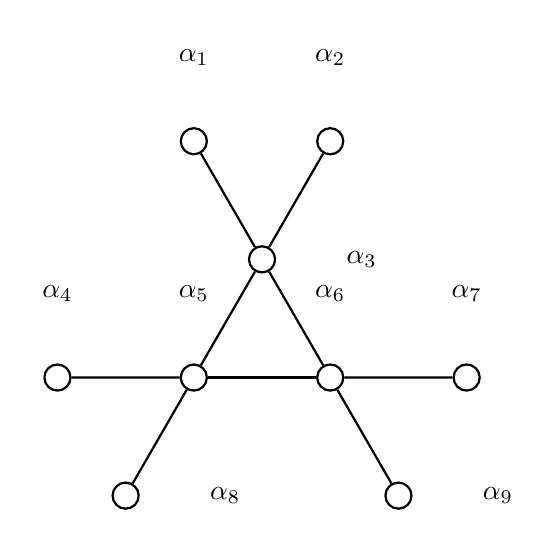
\begin{tikzpicture}
% \node[draw=none] (casenumber) at (-1.5, 3.0) {\emph{Case 7}};
% \draw[help lines,step=0.5] (0,0) grid (14,4);
\def\alabeldist{0.5cm}
\begin{scope}[every node/.style={circle,draw, minimum size=2.4mm}, scale=1.5]
    \begin{scope}
        \begin{scope}[rotate=-60,shift={(0.0, -0.667)}]
                \node[thick, circle, label={[label distance=\alabeldist]90:$\alpha_5$}] (a1) at (0,0) {};
                \node[thick, circle, label={[label distance=\alabeldist]90:$\alpha_4$}] (a2) at (-{tan(30)},-1.0) {};5                \node[thick, circle, label={[label distance=\alabeldist+0.2cm]0:$\alpha_8$}] (a3) at ({tan(30)},-1.0) {};
        \end{scope}
        
        \begin{scope}[shift={(0.0, 0.0)}]
            \begin{scope}[rotate=60,shift={(0.0, -0.667)}]
                    \node[thick, circle, label={[label distance=\alabeldist]90:$\alpha_6$}] (a4) at (0,0) {};
                    \node[thick, circle, label={[label distance=\alabeldist+0.2cm]0:$\alpha_9$}] (a5) at (-{tan(30)},-1.0) {};
                    \node[thick, circle, label={[label distance=\alabeldist]90:$\alpha_7$}] (a6) at ({tan(30)},-1.0) {};
            \end{scope}
        \end{scope}
        
        \begin{scope}[shift={(0.0, 0.0)}]
            \begin{scope}[rotate=180,shift={(0.0, -0.667)}]
                    \node[thick, circle, label={[label distance=\alabeldist+0.2cm]0:$\alpha_3$}] (a7) at (0,0) {};
                    \node[thick, circle, label={[label distance=\alabeldist]90:$\alpha_2$}] (a8) at (-{tan(30)},-1.0) {};
                    \node[thick, circle, label={[label distance=\alabeldist]90:$\alpha_1$}] (a9) at ({tan(30)},-1.0) {};
            \end{scope}
        \end{scope}
    \end{scope}
\end{scope}

\begin{scope}
    \foreach \from/\to in {a1/a2, a3/a1, a7/a8, a9/a7, a4/a5, a6/a4, a1/a7, a7/a4, a4/a1}
        \draw [thick] (\from) -- (\to);
        
    \dashedcontainerthing{a2,a1,a3};
    \dashedcontainerthing{a5,a4,a6};
    \dashedcontainerthing{a8,a7,a9};
\end{scope}
\end{tikzpicture}
    \vspace*{1mm}
    \caption[An instance of 3DR-AS-SMUW in which $u(M^*)=2u(M)$]{An instance of 3DR-AS-SMUW in which $u(M^*)=2u(M)$. The dashed enclosure depicts $M^*$.}
    \label{fig:threed_sr_as_max_welfare_example}
\end{figure}